\documentclass[11pt]{article}
\usepackage[utf8]{inputenc}
\usepackage[margin=0.8in]{geometry}
\usepackage{amsfonts, amsmath}
\usepackage{tikz}
\usepackage[nobreak=false]{mdframed}
\usepackage{pgf}
\usepackage{mathtools}
\usepackage{bbm}
\usepackage{graphicx}
\usepackage{url}
\usepackage{enumerate}
\usepackage{amsthm,amssymb}
\usepackage{minted}
\setlength\parindent{0pt}
\newcommand{\solution}{\subsection*{Solution:}}
\newcommand{\Lagr}{\mathcal{L}}

\begin{document}

\title{EE 240C Homework 1}
\author{Vighnesh Iyer}
\date{\today}
\maketitle

\subsection*{Problem 1: Aliasing}
A sinusoidal signal with a frequency of 4 MHz and with second and third harmonics is sampled by a 6 MS/s system.
\begin{enumerate}[a)]
    \item Draw the resulting spectrum. What happens to each of the distortion components?
        Assume that the signal has a fundamental component with amplitude $\alpha$ and 2nd and 3rd harmonics with amplitudes $\beta$ and $\gamma$ respectively.
        The resulting spectrum contains:
        \begin{itemize}
            \item the 4 MHz fundamental aliased to 1 MHz with amplitude $\alpha$
            \item the 8 MHz 2nd harmonic aliased to 2 MHz with amplitude $\beta$
            \item the 12 MHz 3rd harnomic aliased to DC with amplitude $\gamma$
        \end{itemize}
    \item What is the minimum sampling frequency that avoids aliasing?

        $f_s \geq BW \cdot 2 \rightarrow f_s \geq 24 \text{ MS/s}$
\end{enumerate}

\subsection*{Problem 2: Reconstruction}
A discrete time signal with a sample rate of $f_s = 1$ MHz is converted to continuous time using zero-order hold pulses.
\begin{enumerate}[a)]
    \item Plot the frequency response corresponding to reconstruction using zero-order hold pulses for pulse widths of 250ns, 500ns, and 1$\mu$s.

        We derived the amplitude envelope corresponding to using ZOH pulses with pulse width $T_p$ as:
        \begin{align*}
            |H_{ZOH}(f)| = \left| \frac{T_p}{T_s} \frac{\sin(\pi f T_p)}{\pi f T_p}\right|
        \end{align*}
        \begin{center}
        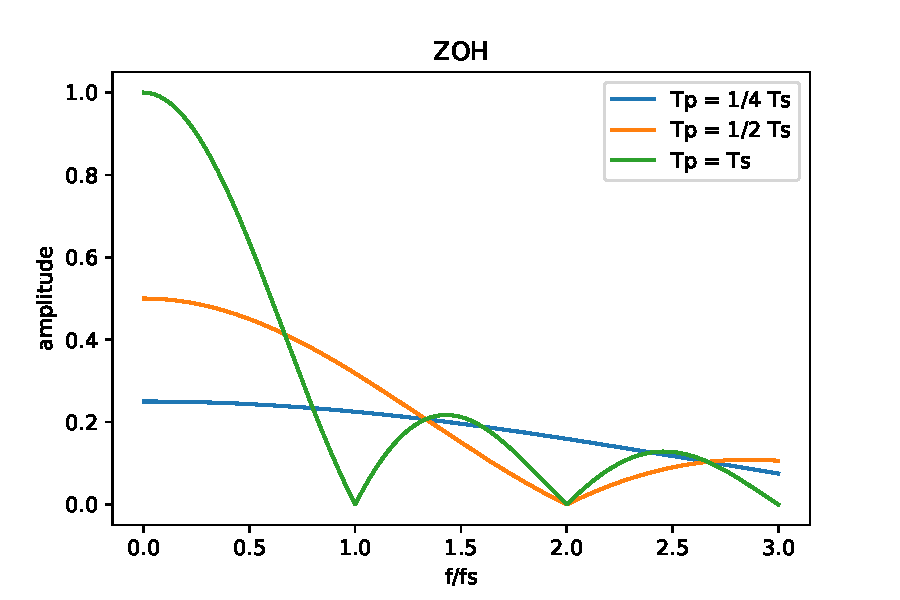
\includegraphics[width=0.5\textwidth]{figs/zoh.pdf}
        \end{center}
    \item Plot the output spectrum up to 2 MHz when a discrete-time sine wave of 200 kHz is converted to continuous-time using a 1$\mu$s zero-order hold pulse.

        This corresponds to convolving the 200 kHz tone with the frequency response of the ZOH pulse.
        The output spectrum has these components:
        \begin{itemize}
            \item $|H_{ZOH}(200 \text{ kHz})|$ at 200 kHz
            \item $|H_{ZOH}(800 \text{ kHz})|$ at 800 kHz
            \item $|H_{ZOH}(1200 \text{ kHz})|$ at 1200 kHz
            \item $|H_{ZOH}(1800 \text{ kHz})|$ at 1800 kHz
        \end{itemize}
\end{enumerate}

\subsection*{Problem 3: ADC DNL and INL}
DNL:
\begin{minted}{python}
hist = [28, 21, 19, 23, 22, 20, 15, 21, 23, 18, 19, 19, 23, 18, 24, 29]
inner_range = sum(hist[1:-1])
wavg = (sum(hist[0:-1]) - hist[0]) / (2**4 - 2)
dnl = (np.array(hist[1:-1]) - wavg) / wavg
print(dnl)
print(np.max(dnl))
print(np.min(dnl))
\end{minted}
\begin{minted}{text}
[ 0.03157895 -0.06666667  0.12982456  0.08070175 -0.01754386 -0.26315789
  0.03157895  0.12982456 -0.11578947 -0.06666667 -0.06666667  0.12982456
 -0.11578947  0.17894737]
0.1789473684210526
-0.26315789473684215
\end{minted}

INL:
\begin{minted}{python}
inl = np.cumsum(dnl)
print(np.max(inl))
print(np.min(inl))
\end{minted}
\begin{minted}{text}
0.17543859649122795
-0.1929824561403512
\end{minted}

\subsection*{Problem 4: ADC DNL and INL}
\begin{enumerate}[a)]
    \item Monotonic ADC with output codes 0, 1, 2, $\dots, M$. Show:
        \begin{align*}
            \text{INL}(k) &= \sum_{i=1}^{k-1} \text{DNL}(i) \\
            &= \sum_{i=1}^{k-1} \frac{\text{Step}(k) - \text{Step}_{\text{avg}}}{\text{Step}_{\text{avg}}} \\
            &= \sum_{i=1}^{k-1} \frac{\text{T}(k+1) - \text{T}(k) - \text{Step}_{\text{avg}}}{\text{Step}_{\text{avg}}} \\
            &= \frac{1}{\text{Step}_{\text{avg}}} T(n) - T(0) - (n-2)\text{Step}_{\text{avg}} \\
            &= \frac{T(k) - T_{uniform}(k)}{W_{avg}}
        \end{align*}

    \item Sum of DNLs is 0.

        We know INL(M) = 0.
        \begin{align*}
            \text{INL}(M) = 0 = \sum_{i=1}^{M-1} \text{DNL}(i)
        \end{align*}
\end{enumerate}
\end{document}
